% \section{JavaScript}

Als JavaScript 1997 veröffentlicht und in den NetScape Navigator integriert wurde, gab es Bedenken, dass das Öffnen einer Webseite dem Betreiber erlaubt Code auf dem System eines Nutzers auszuführen. Damit dies nicht eintritt, wurde der JavaScript Ausführungskontext in eine virtuelle Umgebung integriert, einer sog. Sandbox \cite{LearningJavaScript}.

Die JavaScript-Sandbox des Browsers schränkt den Zugriff auf das Dateisystem ein. Darüber hinaus sind auch keine Zugriffe auf native Bibliotheken oder die Ausführung von nativem Code möglich \cite{TheSpyInTheSandbox}. Um z. B. Daten beim Client zu speichern oder auch Videos abzuspielen bieten Browser eigene Schnittstellen hierfür an.

\nomenclature[Fachbegriff]{CORS}{Cross-Origin Resource Sharing}
\nomenclature[Fachbegriff]{Ajax}{Asynchronous JavaScript and XML}
\nomenclature[Fachbegriff]{W3C}{World Wide Web Consortium}
\nomenclature[Fachbegriff]{XHR}{XMLHttpRequest}

1999 nahm Microsoft im Internet Explorer 5.0 eine neue Funktion in ihre JavaScript-Umgebung auf: Asynchronous JavaScript and XML (Ajax) \cite{MDNAjax}. Ajax erlaubt die Datenabfrage von Webservern mittels JavaScript. Hierdurch können Inhalte auf Webseiten dynamisch abgefragt und dargestellt werden, wofür zuvor ein weiterer Seitenaufruf notwendig war. Das Konzept wurde kurz darauf von allen damals gängigen Browsern übernommen. Jedoch fand erst mit der Standardisierung von Ajax durch das W3C \cite{TheXMLHttpRequestObject} das Konzept Anklang bei Entwicklern \cite{AngularForEnterpriseReadyWebApplications} \cite{FinkIntroducingSPAs} und ist seitdem der Grundstein für unser dynamisches und interaktives Web \cite{ResearchOnAJAXTechnology}.

Durch die Unterstützung von Ajax wurden Webanwendungen immer beliebter. Entwickler beklagten jedoch vermehrt, dass Browser die Abfragen von JavaScript nur auf dem bereitstellenden Webserver, also \enquote{same-origin}, erlauben \cite{CrossSiteXHRWithCORS}. Um eine größere Flexibilität zu ermöglichen, wurde im selben Jahr der Standardisierung von Ajax ein erster Entwurf zur Absicherung beim Abrufen domänenfremder Ressourcen eingereicht \cite{AuthorizingCORS}, das sogenannte Cross-Origin Resource Sharing.

Über die Jahre wurde der JavaScript-Standard immer umfangreicher, was Entwicklern erlaubte mächtige Werkzeuge sowie Frameworks zu entwickeln, welche die Erstellung von Webanwendungen vereinfachen. Mit Webanwendungen war es nun möglich, einen großen Teil der Funktionalitäten eines Produktes im Browser auszuführen.

\subsection{Content-Security-Policy}

\nomenclature[Fachbegriff]{CSP}{Content-Security-Policy}
\nomenclature[Fachbegriff]{XSS}{Cross-Site-Scripting}

Im Browser haben Entwickler die Möglichkeit zu bestimmen, welche Funktionalitäten einer Webanwendung zur Verfügung stehen sollen und wie diese vom Browser einzuschränken sind. Diese Funktion heißt Content-Security-Policy (CSP) und dient unter anderem dem Schutz vor Cross-Site-Scripting. Mit der CSP kann eine Webanwendung beschränken, welche Funktionalitäten in JavaScript verfügbar sind und von wo aus Skripte und Daten geladen werden dürfen \cite{MDNContentSecurityPolicy}. Weiterhin kann eingerichtet werden, dass bei einem Versuch diese CSP-Regeln zu umgehen, darüber Bericht erstattet wird.

\subsection{Cross-Origin Resource Sharing (CORS)}

Cross-Origin Resource Sharing (CORS) \cite{AuthorizingCORS} entwickelte sich aus dem Wunsch von Entwicklern, nicht auf einen einzelnen Webserver beschränkt zu sein. Eine Einschränkung, die eingeführt wurde, um Nutzer vor Missbrauch zu schützen \cite{BrowserProtectionAgainstCSRF}. CORS lockert diese Einschränkung unter Berücksichtigung sicherheitskritischer Aspekte. Das Konzept von CORS stellt sicher, dass aus JavaScript heraus keine Daten von Webservern angefragt werden können, welche nicht explizit der Anfrage zustimmen \cite{MDNCORS}.

Wie eine \enquote{cross-origin} Ajax-Anfrage nach dem Konzept von CORS gehandhabt wird, ist in \autoref{fig:cors-workflow} dargestellt. Wenn eine HTTP-Anfrage nicht \enquote{simple}\footnotemark{} ist, führt der Browser einen sogenannten \enquote{Preflighted Request} aus, bei dem vor der eigentlichen Anfrage eine zusätzliche OPTIONS-Anfrage gesendet wird. Bestätigt nun der Webserver in seiner Antwort auf die OPTIONS-Anfrage, dass die Anfrage erlaubt ist, wird die eigentliche Ajax-Anfrage ausgeführt. Ansonsten schlägt die Anfrage fehl und wird in JavaScript aus Sicherheitsgründen ohne detaillierte Beschreibung gemeldet \cite{MDNCORS}.

\footnotetext{\enquote{simple} ist sie, wenn 1. die Methode GET, HEAD oder POST entspricht; 2. keine benutzerdefinierten Header enthalten sind; und 3. bei POST-Anfragen der \enquote{Content-Type} einem dieser Werte entspricht: \enquote{application/x-www-form-urlencoded}, \enquote{multipart/form-data} oder \enquote{text/plain} \cite{MDNCORS}.}

\begin{figure}[H]
	\centering
	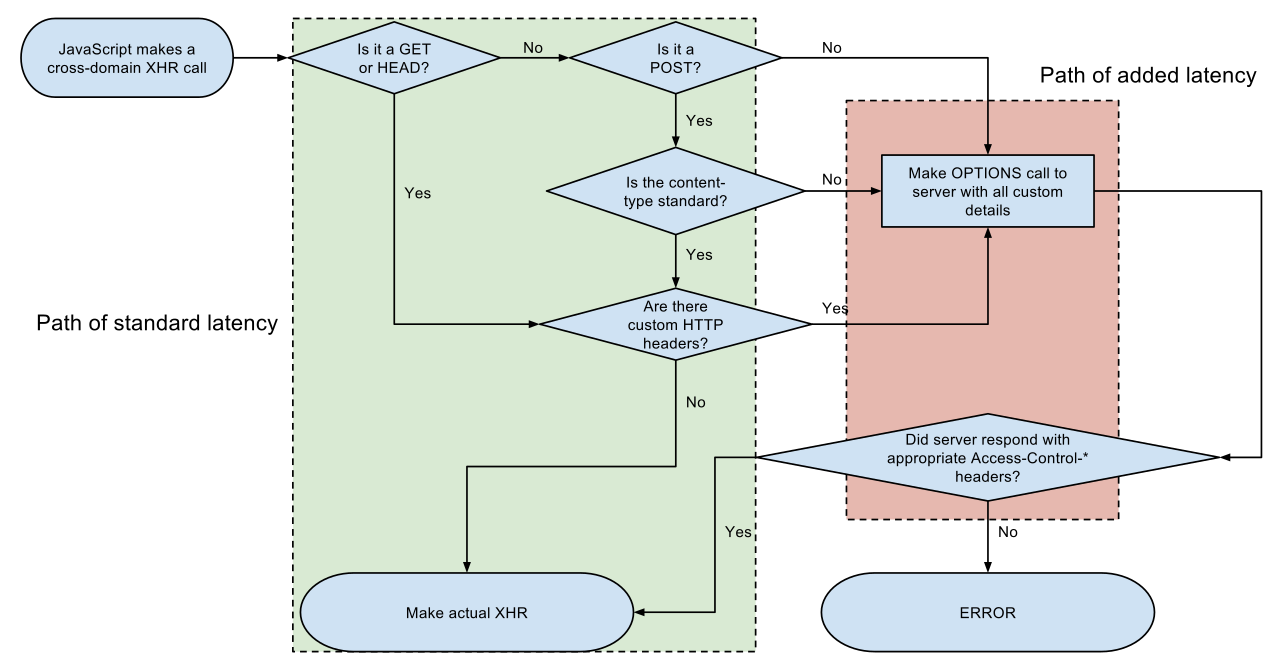
\includegraphics[width=\linewidth]{img/02_theorie/1280px-Flowchart_showing_Simple_and_Preflight_XHR.svg.png}
	\caption{Flowchart über den Ablauf von Ajax-Anfragen mit CORS \cite{FlowchartCORS}}
	\label{fig:cors-workflow}
\end{figure}